\documentclass{article}

% 导入中文宏包
\usepackage{ctex}
\usepackage{array}
\usepackage{caption}
\usepackage{hyperref}
% 设置页面边距
\usepackage{geometry}
\usepackage{graphicx}
\geometry{a4paper, left=2.5cm, right=2.5cm, top=3cm, bottom=3cm}

% 设置标题、作者和日期
\title{Python入门基础和Python视觉应用}
\author{23020007030  关嘉琪}

\begin{document}
	
	% 生成标题、作者和日期
	\maketitle
	
	% 心得报告正文
	\section{实验目的}
	掌握Python的基本语法和编程习惯,能够编写简单的程序。
	
	了解图像处理的基本概念,能够使用Python进行图像读取、显示和保存。
	
	通过实现一个简单的图像分类或识别项目,理解计算机视觉的基本流程。
	
	\section{介绍}
	\subsection{优点}
	1.Python具有清晰的语法结构,对初学者友好,易于上手。
	Python在多个领域都有应用,如数据分析、网络开发、人工智能等,掌握基础后可以轻松转向其他领域。
	
	2.Python视觉应用可以将抽象的算法和理论转化为直观的图像结果,帮助理解
	
	3.命令行可以更加高效、方便、快捷地完成工作,直接对系统进行操作
	\section{实验内容}
	\subsection{Python学习例子10个}
	
	1.print()打印的意思
	print("hello,world")
	
	\noindent
	\begin{minipage}{\linewidth}
		\centering
		% 插入图片
		
\includegraphics[width=0.5\linewidth]{example1.png}
		% 图片标题
		\captionof{figure}{用print来打印想输出的内容}
		\label{fig:example}
	\end{minipage}
	
	
	2.条件语句的使用
	\begin{verbatim}
		x=2 y=3
		if x > y:
			print("x is bigger than y")
		else:
			print("x is not bigger than y")
		
	\end{verbatim}
	
	
	\noindent
	\begin{minipage}{\linewidth}
		\centering
		% 插入图片
		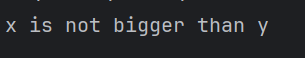
\includegraphics[width=0.5\linewidth]{example2.png}
		% 图片标题
		\captionof{figure}{条件语句输出结果}
		\label{fig:example}
	\end{minipage}
	
	3.循环语句的使用
	\begin{verbatim}
		for i in [1, 2, 3, 4, 5]:
		print(i)
	\end{verbatim}
	
	\noindent
	\begin{minipage}{\linewidth}
		\centering
		% 插入图片
		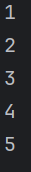
\includegraphics[width=0.5\linewidth,height=17cm]{example3.png}
		% 图片标题
		\captionof{figure}{循环语句的使用}
		\label{fig:example}
	\end{minipage}
	
	4.函数的定义和使用
	\begin{verbatim}
		def greet():
			print("Hello, Python") 
		greet()
	\end{verbatim}
	
	\noindent
	\begin{minipage}{\linewidth}
		\centering
		% 插入图片
		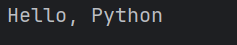
\includegraphics[width=0.5\linewidth]{example4.png}
		% 图片标题
		\captionof{figure}{函数的定义与使用}
		\label{fig:example}
	\end{minipage}
	
	
	
	5.列表的使用
	\begin{verbatim}
		list = [1, 2, 3, 4, 5]
		print(list[0])
	\end{verbatim}
	
	
	\noindent
	\begin{minipage}{\linewidth}
		\centering
		% 插入图片
		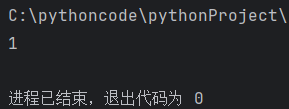
\includegraphics[width=0.5\linewidth]{example5.png}
		% 图片标题
		\captionof{figure}{列表的输出结果}
		\label{fig:example}
	\end{minipage}
	
	6.字典的使用:
	\begin{verbatim}
		person = {
			'名字': '张先生',
			'年龄': 30,
			'城市': '泰安',
			'职业': '计算机工程师'
		}
		
		# 访问字典中的数据
		print(person['名字'])  
		print(person['职业'])
	\end{verbatim}
	
	
	
	\noindent
	\begin{minipage}{\linewidth}
		\centering
		% 插入图片
		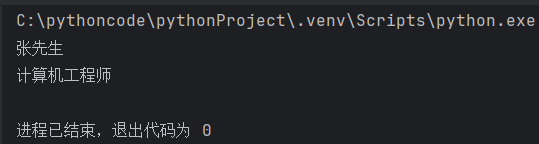
\includegraphics[width=0.5\linewidth]{example6.png}
		% 图片标题
		\captionof{figure}{字典的输出结果}
		\label{fig:example}
	\end{minipage}
	
	7.元组的使用:
	\begin{verbatim}
		tuple= (666, "work", 3.1415)
		print(tuple[1])
	\end{verbatim}
	
	
	\noindent
	\begin{minipage}{\linewidth}
		\centering
		% 插入图片
		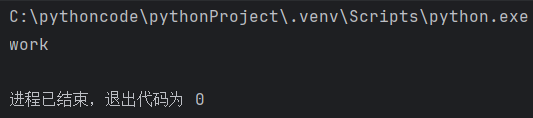
\includegraphics[width=0.5\linewidth]{example7.png}
		% 图片标题
		\captionof{figure}{元组的输出结果}
		\label{fig:example}
	\end{minipage}
	
	
	8.程序和用户的交互:
	\begin{verbatim}
		number = int(input("请输入一个整数:"))
		print("您输入的整数是:", number)
		#int是标明输入的类型
		#number=input()是向number里输入数据
	\end{verbatim}
	
	\noindent
	\begin{minipage}{\linewidth}
		\centering
		% 插入图片
		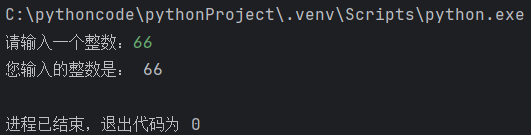
\includegraphics[width=0.5\linewidth]{example8.png}
		% 图片标题
		\captionof{figure}{程序和用户的交互}
		\label{fig:example}
	\end{minipage}
	
	
	
	9. 类的使用:
	\begin{verbatim}
		class Car:
		def __init__(self, make, model, year):
		"""初始化汽车属性"""
			self.make = make
			self.model = model
			self.year = year
			self.odometer_reading = 0  # 汽车里程表初始为0
		
		def describe_car(self):
		"""返回汽车描述信息"""
			return f"{self.year} {self.make} {self.model}"
		
		
		# 创建一个Car实例
		mycar = Car('Toyota', 'Corolla', 2020)
		
		# 打印汽车描述信息
		print(mycar.describe_car())
	\end{verbatim}
	
	\begin{minipage}{\linewidth}
		\centering
		% 插入图片
		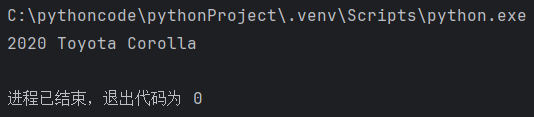
\includegraphics[width=0.5\linewidth]{example9.png}
		% 图片标题
		\captionof{figure}{类的使用}
		\label{fig:example}
	\end{minipage}
	
	
	10.文件的写入和读取
	\begin{verbatim}
		with open('example.txt', 'w') as file:
			file.write('Hello, World!')
		with open('example.txt', 'r') as file:R
			content = file.read()
		print(content)
	\end{verbatim}
	
	
	\noindent
	\begin{minipage}{\linewidth}
		\centering
		% 插入图片
		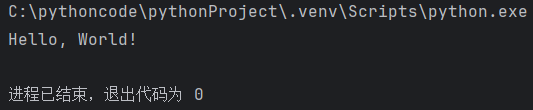
\includegraphics[width=0.5\linewidth]{example10.png}
		% 图片标题
		\captionof{figure}{文件的写入和读取}
		\label{fig:example}
	\end{minipage}
	
	
	
	\subsection{Python视觉应用5个例子}
	1.图像灰度变换
	\begin{verbatim}
		from PIL import Image
		# 读取图像
		image = Image.open('test.png') 
		# 显示图像
		image.show()
		# 转换为灰度图像
		gray_image = image.convert('L')
		gray_image.show()
	\end{verbatim}
	
	\noindent
	\begin{minipage}{\linewidth}
		\centering
		% 插入图片
		
\includegraphics[width=0.5\linewidth]{test.png}
		% 图片标题
		\captionof{figure}{灰度变换前}
		\label{fig:example}
	\end{minipage}
	
	\noindent
	\begin{minipage}{\linewidth}
		\centering
		% 插入图片
		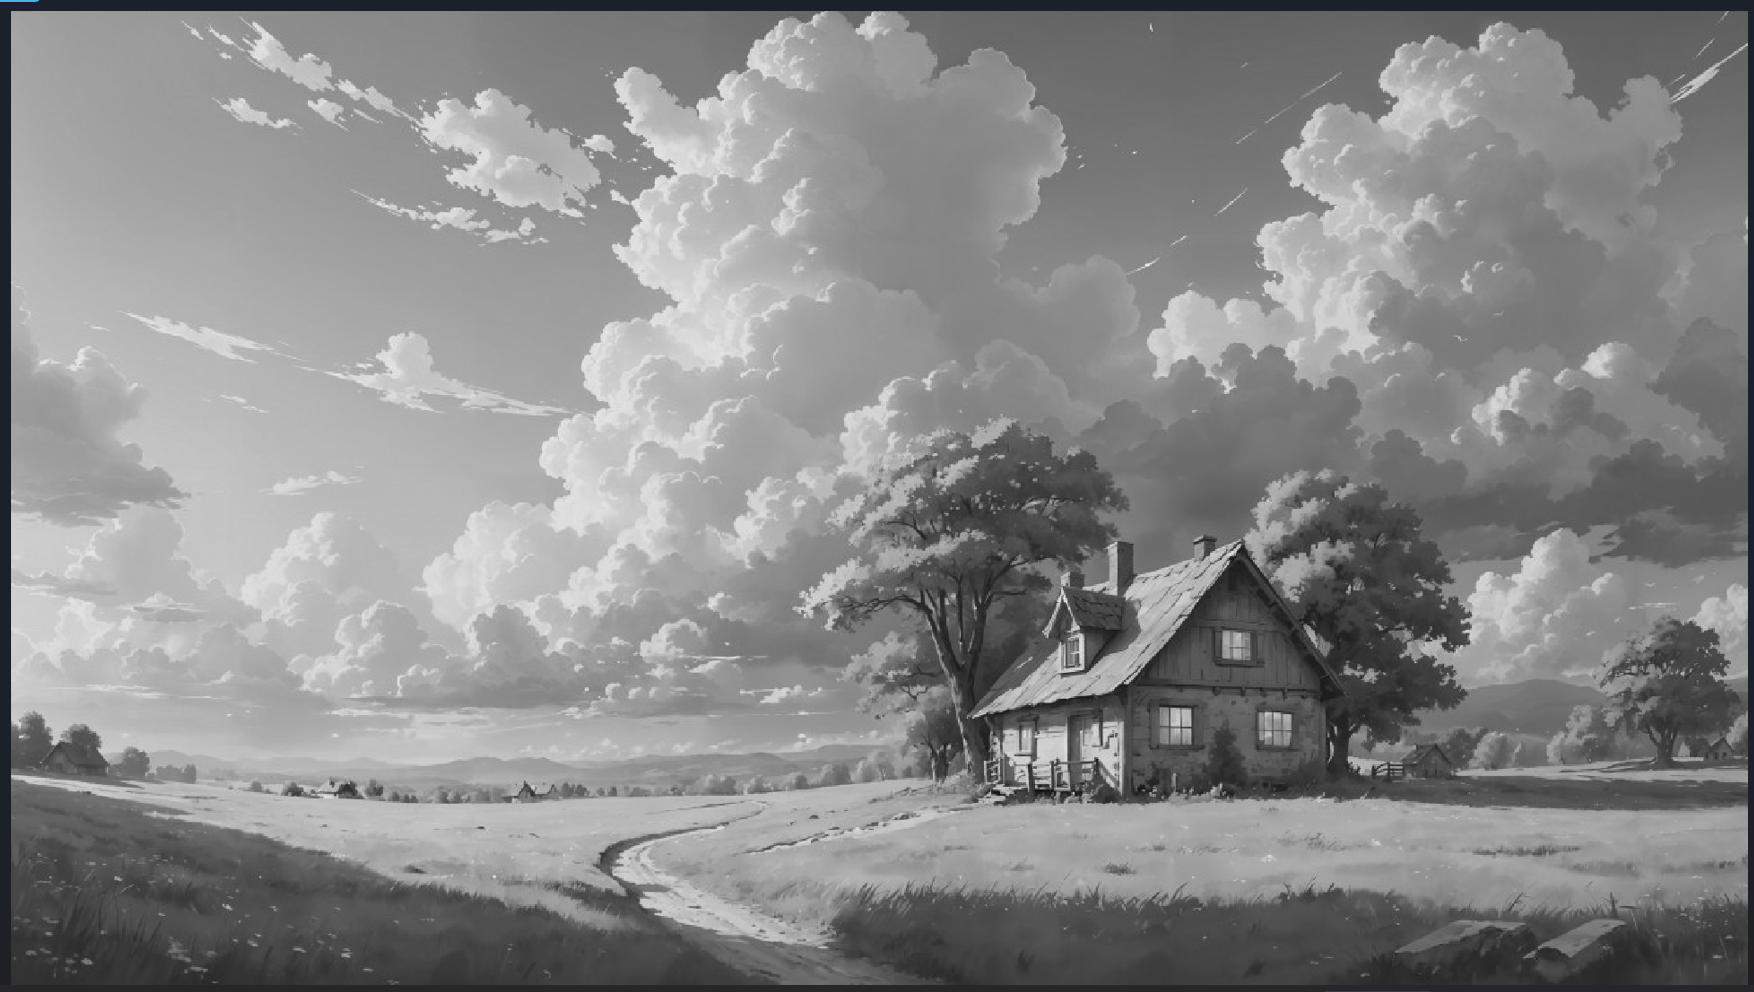
\includegraphics[width=0.5\linewidth]{completed.png}
		% 图片标题
		\captionof{figure}{灰度变换后}
		\label{fig:example}
	\end{minipage}
	
	2.利用Matplotlib完成折线图的绘制
	\begin{verbatim}
		import matplotlib.pyplot as plt
		import numpy as np
		x = np.linspace(0, 10, 100)  # 生成从0到10的100个点
		y = np.sin(x) + np.random.normal(0, 0.1, 100)  # 生成正弦曲线并添加一些随机噪声
		# 创建图形和轴
		plt.figure(figsize=(10, 6))  # 设置图形的大小
		plt.plot(x, y, label='sin(x) + noise', color='blue')  # 绘制折线图
		# 添加标题和标签
		plt.title('Simple Plot')
		plt.xlabel('X axis')
		plt.ylabel('Y axis')
		# 添加图例
		plt.legend()
		# 显示网格(可选)
		plt.grid(True)
		# 显示图形
		plt.show()
	\end{verbatim}
	
	\noindent
	\begin{minipage}{\linewidth}
		\centering
		% 插入图片
		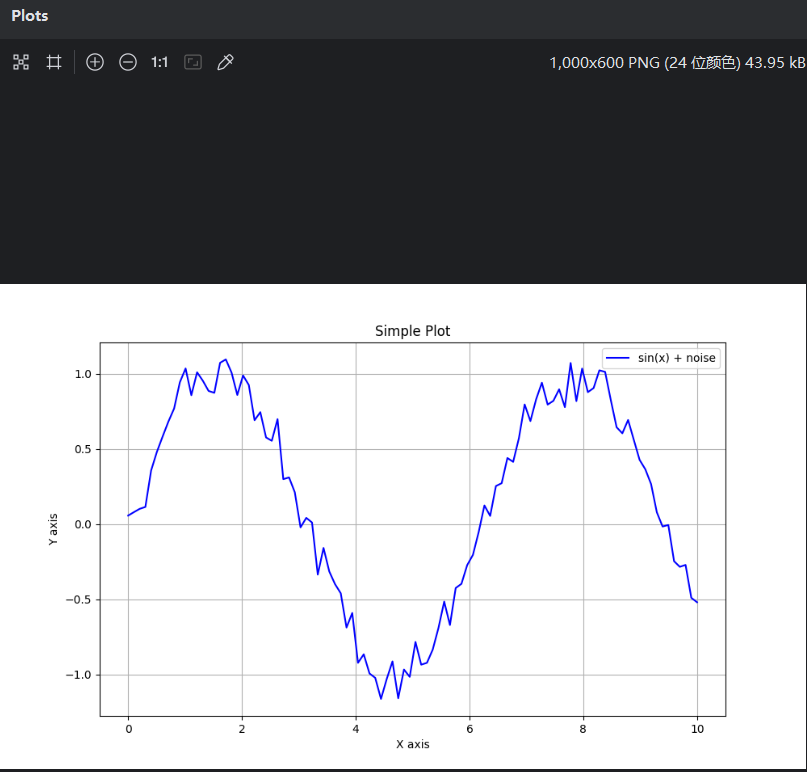
\includegraphics[width=0.5\linewidth]{zhexian.png}
		% 图片标题
		\captionof{figure}{绘制的折线图}
		\label{fig:example}
	\end{minipage}
	
	3.图像模糊
	\begin{verbatim}
		from PIL import Image
		import numpy as np
		import cv2
		# 读取图像
		image = Image.open('测试图片.png')
		# 转换图像为numpy数组
		image_np = np.array(image)
		# 应用均值模糊
		blurred_image_np = cv2.blur(image_np, (5, 5))
		# 转换numpy数组回PIL图像
		blurred_image = Image.fromarray(blurred_image_np)
		# 显示原始图像和均值模糊后的图像
		image.show()
		blurred_image.show()
	\end{verbatim}
	
	\noindent
	\begin{minipage}{\linewidth}
		\centering
		% 插入图片
		
\includegraphics[width=0.5\linewidth]{test.png}
		% 图片标题
		\captionof{figure}{图像模糊之前如下:}
		\label{fig:example}
	\end{minipage}
	
	\noindent
	\begin{minipage}{\linewidth}
		\centering
		% 插入图片
		
\includegraphics[width=0.5\linewidth]{mohu.png}
		% 图片标题
		\captionof{figure}{图像模糊之后如下:}
		\label{fig:example}
	\end{minipage}
	
	4.图像缩放
	\begin{verbatim}
		import matplotlib.pyplot as plt
		# 读取图像
		image = plt.imread('测试图片.png')
		# 设置缩放比例
		scale_percent = 50  
		width = int(image.shape[1] * scale_percent / 100)
		height = int(image.shape[0] * scale_percent / 100)
		# 创建一个缩放后的图像
		resized_image = image[0:height, 0:width]
		# 显示缩放后的图像
		plt.imshow(resized_image)
		plt.axis('off')  # 不显示坐标轴
		plt.show()
		
	\end{verbatim}
	
	\noindent
	\begin{minipage}{\linewidth}
		\centering
		% 插入图片
		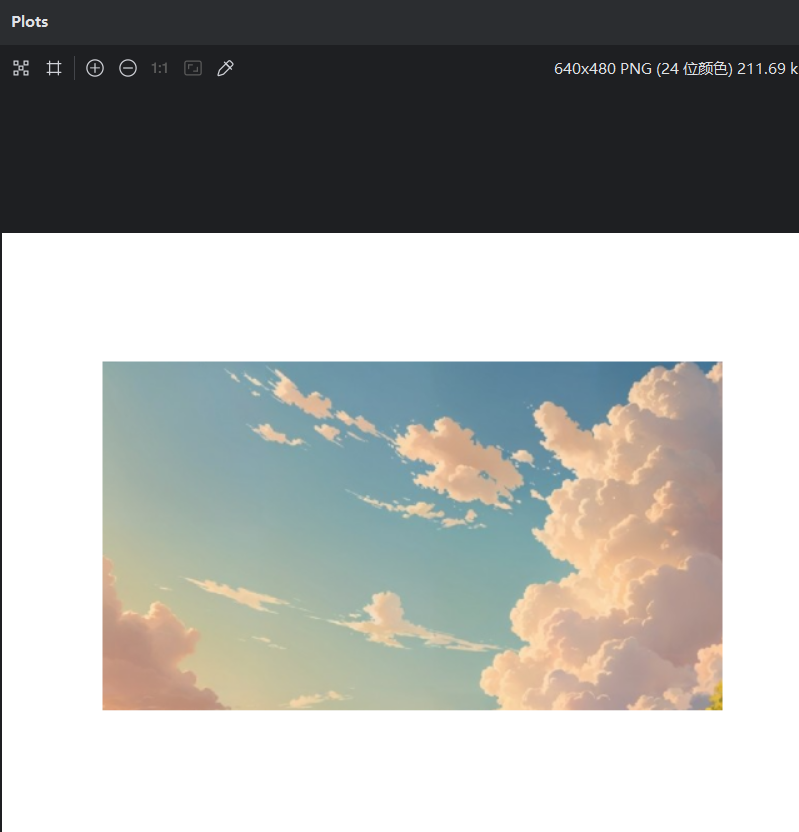
\includegraphics[width=0.5\linewidth]{suofang.png}
		% 图片标题
		\captionof{figure}{缩放后的图片}
		\label{fig:example}
	\end{minipage}
	
	5.缩略图绘制
	\begin{verbatim}
		from PIL import Image
		# 读取原始图像
		original_image = Image.open('测试图片.png')  # 替换为您的图像路径
		# 设置缩略图的比例因子
		thumbnail_ratio = 0.25  # 缩略图尺寸是原始尺寸的25%
		# 创建缩略图
		thumbnail = original_image.resize((int(original_image.width * thumbnail_ratio), int(original_image.height * thumbnail_ratio)), Image.BICUBIC)
		# 显示原始图像和缩略图
		original_image.show()
		thumbnail.show()
	\end{verbatim}
	
	\noindent
	\begin{minipage}{\linewidth}
		\centering
		% 插入图片
		
\includegraphics[width=0.5\linewidth]{suolue.png}
		% 图片标题
		\captionof{figure}{缩略图绘制}
		\label{fig:example}
	\end{minipage}
	
	\subsection{命令行学习5个例子}
	1.创建文件夹:
	\begin{verbatim}
		mkdir new_folder
	\end{verbatim}
	\noindent
	\begin{minipage}{\linewidth}
		\centering
		% 插入图片
		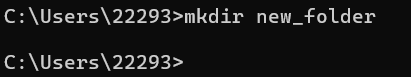
\includegraphics[width=0.5\linewidth]{example11.png}
		% 图片标题
		\captionof{figure}{创建文件夹}
		\label{fig:example}
	\end{minipage}
	
	2.删除文件夹:
	\begin{verbatim}
		rmdir /s /q folder_name
	\end{verbatim}
	
	
	\noindent
	\begin{minipage}{\linewidth}
		\centering
		% 插入图片
		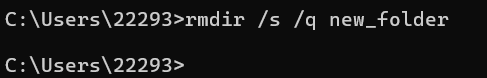
\includegraphics[width=0.5\linewidth]{example12.png}
		% 图片标题
		\captionof{figure}{删除文件夹}
		\label{fig:example}
	\end{minipage}
	
	3.文本文件的建立与写入
	\begin{verbatim}
		echo "Hello, World!" > hello.txt
	\end{verbatim}
	
	\noindent
	\begin{minipage}{\linewidth}
		\centering
		% 插入图片
		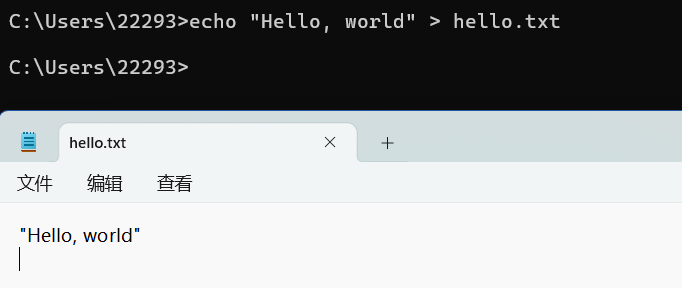
\includegraphics[width=0.5\linewidth]{example13.png}
		% 图片标题
		\captionof{figure}{文本文件的建立与写入}
		\label{fig:example}
	\end{minipage}
	
	4.查看文件内容
	\begin{verbatim}
		type hello.txt
	\end{verbatim}
	
	\noindent
	\begin{minipage}{\linewidth}
		\centering
		% 插入图片
		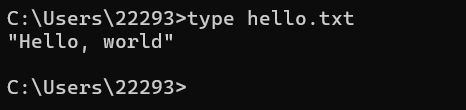
\includegraphics[width=0.5\linewidth]{example14.png}
		% 图片标题
		\captionof{figure}{列表的输出结果}
		\label{fig:example}
	\end{minipage}
	
	5.查看内存信息
	\begin{verbatim}
		wmic memorychip list brief
	\end{verbatim}
	
	\noindent
	\begin{minipage}{\linewidth}
		\centering
		% 插入图片
		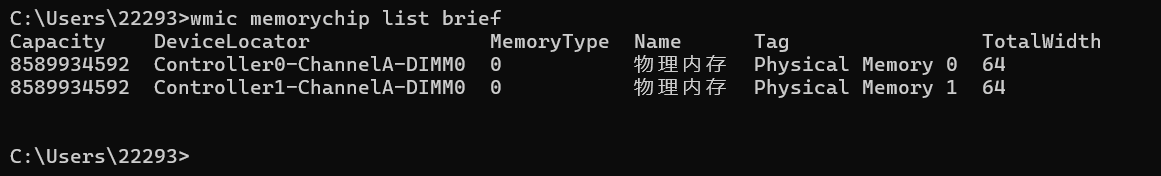
\includegraphics[width=0.5\linewidth]{example15.png}
		% 图片标题
		\captionof{figure}{内存信息}
		\label{fig:example}
	\end{minipage}
	
	\section{实验总结}
	在学习Python的过程中,我发现这是一种更加简洁和高效的编程语言,其语法易于掌握。Python的应用范围广泛,涵盖了多个领域,包括:Web开发、数据分析、人工智能、自动化脚本、游戏开发...
	我计划深入学习Python,以提升我的编程能力。
	利用Python的可视化功能,我能够将抽象的数据转化为直观的图形,这使得信息更加易于理解。
	同时,命令行工具教会了我如何高效地与计算机系统进行交互,从而快速完成各种任务。
	今后我将充分利用这两种工具来处理数据和文件,以提高工作效率。

	github路径:
	\url{https://github.com/Joyceapple/repo/tree/882ed1e61086de8416aa3aab2c9ee2686ee77e82/python}
\end{document}
